\section{Agile methodology and project organization}

For the organization of the project, we used Github Project.
One of the great advantages of this tool is its direct integration with the code.

First, we defined the use cases in Github Issues.
This allowed us to define the functionalities of our project and break them down into smaller tasks.
It is a perfect integration of the agile method, which allows the project to be broken down and assigned to team members.

\begin{figure}[h]
    \centering
    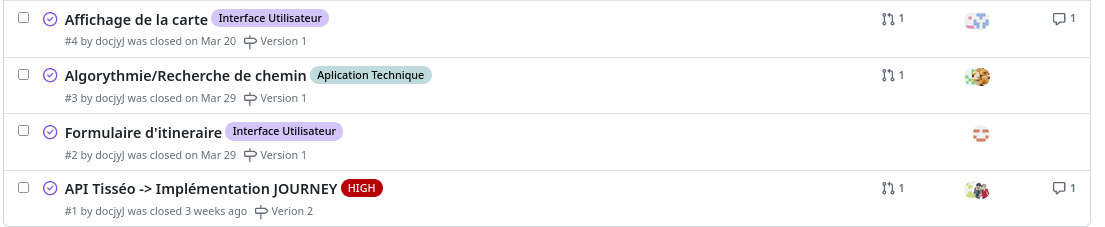
\includegraphics[width=0.8\textwidth]{img/GitHubUseCase}
    \caption{Example use case on GitHub Issue}
    \label{fig:GitHubUseCase}
\end{figure}

Then we had to bring together the different parts of the project.
Once again, Github Project allowed us to integrate this step as best as possible.
Via a pull request, we had a discussion space directly on the code.
For example in figure \ref{fig:GitHubPullRequest}, we can discuss an implementation.
These discussions allow the code to be properly integrated.

\begin{figure}[h]
    \centering
    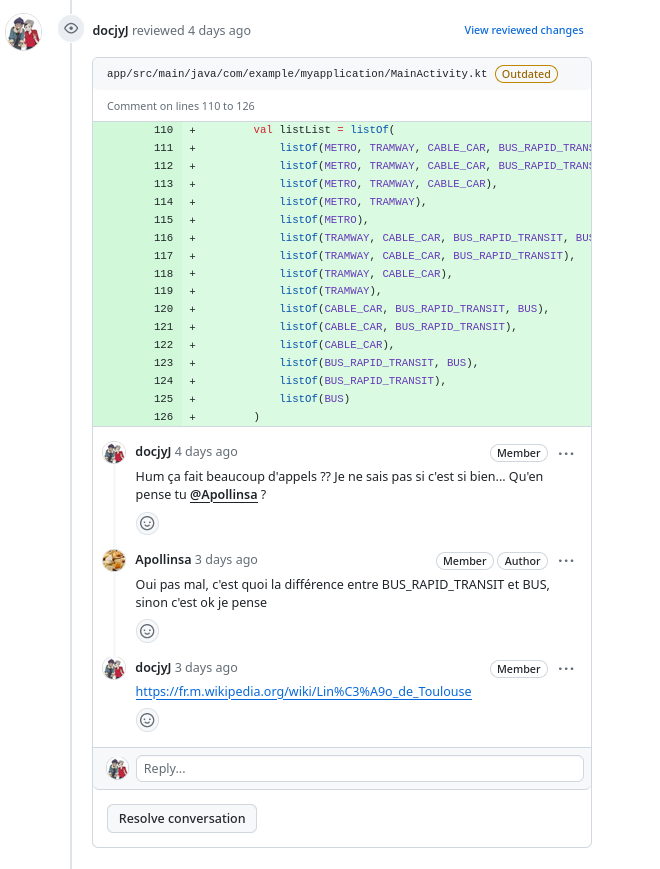
\includegraphics[width=0.4\textwidth]{img/GitHubDiscuss}
    \caption{Example of a discussion in a Pull Request on GitHub}
    \label{fig:GitHubPullRequest}
\end{figure}

\newpage

Then, Github Project allowed us to track the various unforeseen bugs.
Each person is free to add a bug, and we add it to the current sprint or for later depending on its criticality.
Even if adding tasks during the sprint is not recommended, it allowed us to adapt to the project for urgent situations.

\begin{figure}[h]
    \centering
    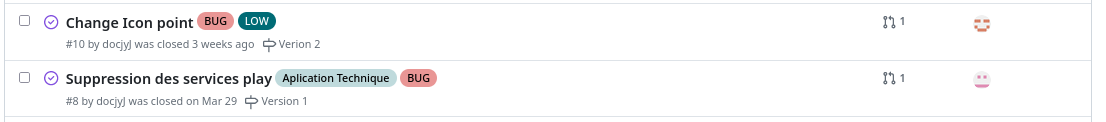
\includegraphics[width=0.8\textwidth]{img/GitHubBug}
    \caption{Example of bug reported on GitHub}
    \label{fig:GitHubBug}
\end{figure}

These three elements allow perfect integration of the agile method into our project.
In addition, GitHub project also provides several views that allow you to monitor the progress of the project.
All of these views are configurable based on the assigned sprint, labels, people, etc.
Formatting, Kanban in figure \ref{fig:GitHubKanban}, Gantt in figure \ref{fig:GitHubGant} or table,
are available to monitor the progress of the project.


\begin{figure}[h]
    \centering
    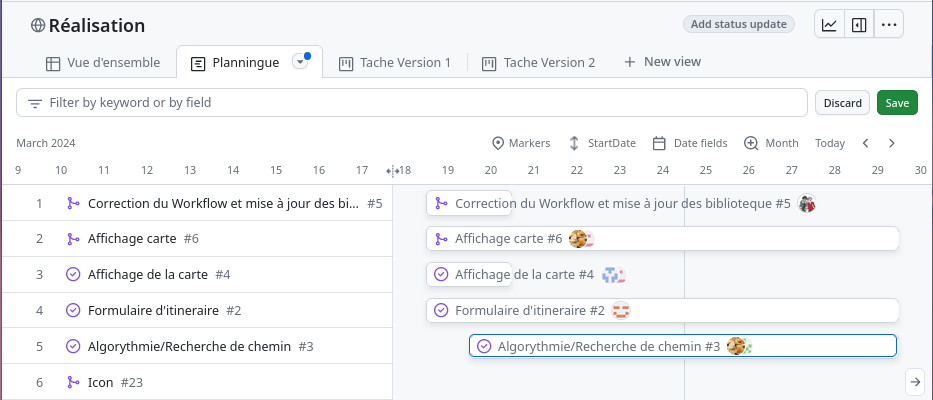
\includegraphics[width=0.8\textwidth]{img/GitHubGant}
    \caption{GitHub Project Gantt view}
    \label{fig:GitHubGant}
\end{figure}

\begin{figure}[h]
    \centering
    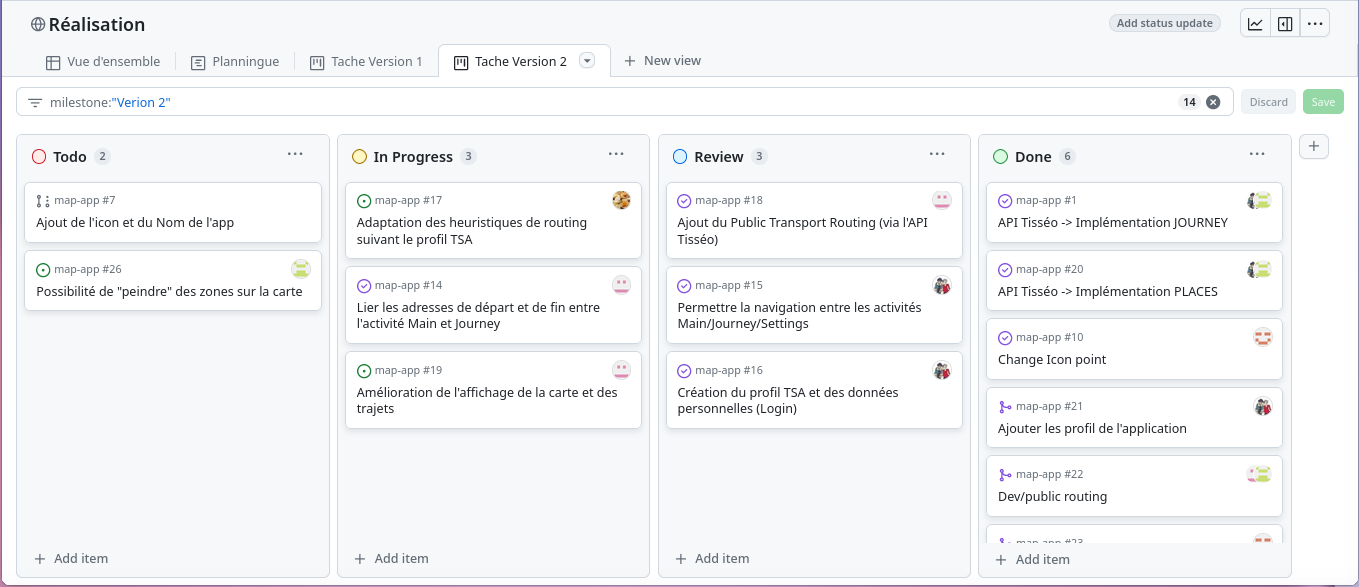
\includegraphics[width=0.8\textwidth]{img/GitHubKanban}
    \caption{GitHub Project Kanban view}
    \label{fig:GitHubKanban}
\end{figure}

We can also divide the different sprints via milestones.
This allows you to set goals with a deadline.


\newpage

Continuous integration tools like GitHub Action allow you to verify the code with each push,
but also having to be able to download an artifact.
This artifact allows us to do tests outside the development environment.
This is a great asset for code quality and development speed.


\begin{figure}[H]
    \centering
    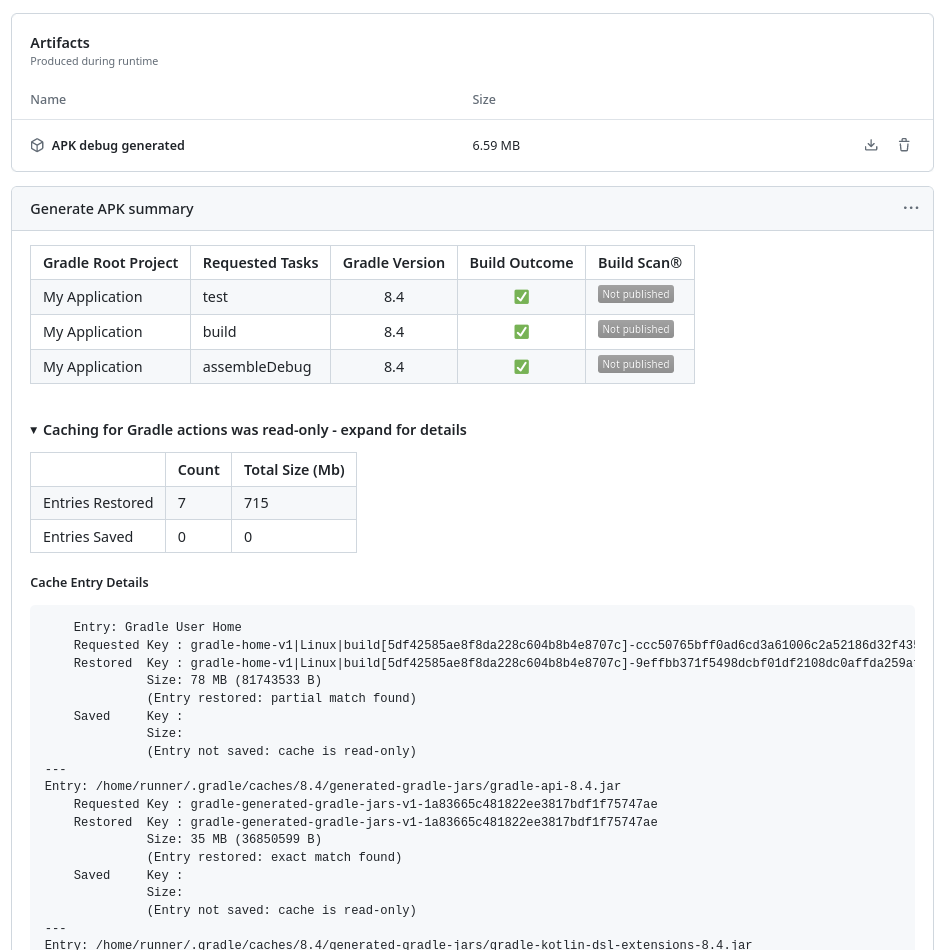
\includegraphics[width=0.4\textwidth]{img/GitHubAction}
    \caption{Workflow example with GitHub Action, with the downloadable artifact}
    \label{fig:GitHubAction}
\end{figure}


Even though GitHub Project is not as powerful as tools like Jira,
the centralization of project management accompanied by its extreme flexibility and modularity make it a perfect tool
for a modern agile method.
